\title{TTL Digital Circuits}

\begin{document}
\section{Diode Logic}

\begin{frame}{Diode logic}
  \begin{definition}
    A \alert{diode} is a semiconductor device that allows current to flow in only one direction.
  \end{definition}
  \begin{center}
    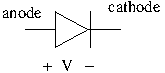
\includegraphics{Diode}
  \end{center}
  \begin{itemize}
    \item Current can flow from the anode to the cathode.
    \item If V is negative, the diode is \alert{reverse biased} and no current flows through the diode.
    \item If V is nonnegative, the diode is \alert{forward biased} and current flows through the diode.
  \end{itemize}
  Diodes can be used to create a number of different logic gates.
\end{frame}

\section{Bipolar Junction Transistors}

\begin{frame}{Bipolar junction transistors}
  \begin{definition}
    For our purposes a \alert{bipolar junction transistor} is a current controlled switch.
  \end{definition}
  \begin{center}
    An npn transistor:\\
    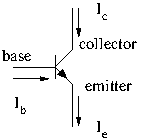
\includegraphics{BipolarJunctionTransistor}
  \end{center}
  \begin{itemize}
    \item If $I_b$ is zero, no current flows from the collector to the emitter.
    \item If $I_b$ is positive, the emitter current is given by $I_e = I_b + I_c$.
  \end{itemize}
\end{frame}

\begin{frame}{Common-emitter configuration}
  \begin{center}
    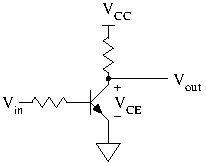
\includegraphics{CommonEmitter}
  \end{center}
  \begin{itemize}
    \item If $V_{in}$ is LOW, the transistor is cut off, so $V_{out}$ is HIGH.
    \item If $V_{in}$ is HIGH, the transistor is saturated, so $V_{out}$ is LOW.
  \end{itemize}
  Saturation can cause the circuit to be slow, so typically, a Schottky diode is used to prevent saturation.
\end{frame}

\section{Transistor-Transistor Logic}

\begin{frame}{Transistor-transistor logic}
  Transistor-transistor logic is usually called TTL.
  \begin{block}{Simple TTL Description}
    \begin{itemize}
      \item TTL uses diode logic and bipolar junction transistors to create logic gates.
      \item TTL functionality is generally the same a CMOS.
      \item TTL circuits have different electrical behavoir.  Typically they require and allow more current flow.
    \end{itemize}
  \end{block}
\end{frame}

\begin{frame}{TTL logic levels}
  \begin{center}
    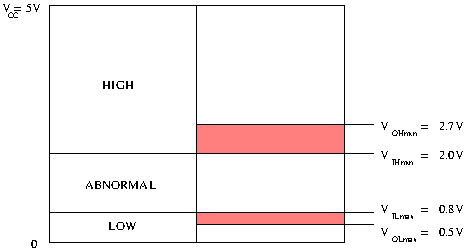
\includegraphics{TTLLogicLevels}
  \end{center}
\end{frame}

\begin{frame}{TLL fanout}
  \begin{block}{TTL Fanout}
    \begin{itemize}
      \item Recall that TTL circuits require more current than CMOS circuits.
      \item Therefore, TTL the fanout for TTL circuits driving other TLL circuits is usually small.
      \item Check the data sheet for details specific to a given device.
    \end{itemize}
  \end{block}
  Overloading a TLL fanout can destroy a device and even burn someone, so exercise caution.
\end{frame}

\end{document}
